\include{template}
\cfoot{} %% if no page number is needed

\begin{document}

\begin{header}
Activité 3 -- Composition des mélanges
\end{header}

\begin{enumerate}
\item Pour une nouvelle création, un bijoutier prépare un alliage d'or 9 carats composé de \unit{9}{\gram} d'or et \unit{15}{\gram} d'autres métaux comme l'argent, le cuivre et le nickel.
\begin{multicols}{2}
\begin{enumerate}
\item La proportion en masse d'or dans l'alliage est $\frac{9}{15}$ ;

\item La proportion en masse d'or dans l'alliage est $\frac{9}{24}$ ;

\item le pourcentage massique d'or dans l'alliage est \unit{37{,}5}{\%} ;

\item le pourcentage massique d'or dans l'alliage est \unit{60}{\%} ;
\end{enumerate}
\end{multicols}

\item On prépare une vinaigrette en mélangeant \unit{7}{mL} à \unit{3}{mL} de vinaigre.
Quelle est la composition volumique de ce mélange ?
\begin{multicols}{2}
\begin{enumerate}
\item \unit{120}{\%} d'huile et \unit{30}{\%} de vinaigre ;

\item \unit{50}{\%} d'huile et \unit{50}{\%} de vinaigre ;

\item \unit{70}{\%} d'huile et \unit{30}{\%} de vinaigre ;

\item \unit{70}{\%} d'huile et \unit{43}{\%} de vinaigre ;
\end{enumerate}
\end{multicols}

\item Un quatre-quarts est un gâteau qui se cuisine en mélangeant un volume égal de farine, d'œufs, de sucre et de beurre :
\begin{multicols}{2}
\begin{enumerate}
\item la proportion de sucre dans la pâte est $\frac{1}{2}$ ;

\item il est composé à \unit{25}{\%} en volume de sucre ;

\item le nom du gâteau est bien mérité !

\item la proportion de sucre dans la pâte est $\frac{1}{4}$ ;

\item il est composé à \unit{50}{\%} en volume de sucre ;

\item le nom du gâteau est mal choisi !
\end{enumerate}
\end{multicols}

\item Les expériences de Lavoisier sur l'air montrent qu'un volume de \unit{0{,}8}{\liter} d'air contient \unit{0{,}168}{\liter} de dioxygène et \unit{0{,}624}{\liter} de diazote.
Donner le pourcentage volumique de dioxygène et de diazote dans l'air.

\item Après un une séance de TP, un élève étourdi laisse le flacon de sulfate de cuivre (initialement blanc) et la bouteille d'eau de chaux ouverts dans un coin de la salle.
À son retour quelques jours plus tard, il constate que le sulfate de cuivre est devenu bleu et que l'eau de chaux s'est troublée.
Que peut-on en déduire ?
\end{enumerate}

\begin{figure}[h]
\center
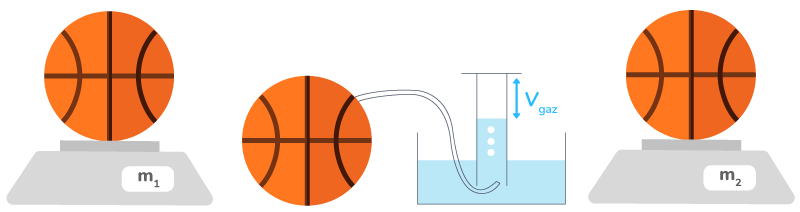
\includegraphics[scale=0.5]{images/masse_volumique_air.png}
\end{figure}

Un élève souhaite mesurer la masse volumique de l'air.
Pour cela, à l'aide d'une balance précédemment tarée, il mesure la masse d'un ballon gonflé d'air sur une balance et lit \unit{598{,}6}{\gram} (masse $m_1$ sur la balance).
Il dégonfle ensuite légèrement le ballon en mesurant le volume d'air qui s'en échappe par déplacement d'eau.
Il lit sur l'éprouvette graduée un volume de \unit{2{,}00}{\liter} (volume $V_\mathrm{gaz}$).
Finalement, il pèse à nouveau le ballon et constate que la masse a diminué : il lit \unit{596{,}2}{\gram} (masse $m_2$).

\begin{enumerate}
\setcounter{enumi}{5}
\item Quelle est la masse d'air qui s'est échappée du ballon quand l'élève l'a dégonflé ?
\item En déduire la masse volumique de l'air, exprimée en g/L ?
\end{enumerate}



\end{document}